%\documentclass[runningheads,a4paper]{llncs}
\documentclass[10pt, conference, compsocconf]{IEEEtran}
\usepackage{amssymb}
%\setcounter{tocdepth}{3}
\usepackage{graphicx}
\usepackage{algorithm}
\usepackage{algorithmic}
\usepackage{comment}
\usepackage{hyperref}
\usepackage{subfigure}
\usepackage{url}
\usepackage{multirow}
\usepackage{amsmath}
\usepackage{xcolor,colortbl}
\usepackage{float}
\usepackage{capt-of}
\usepackage{natbib}

%\newcommand{\keywords}[1]{\par\addvspace\baselineskip
%\noindent\keywordname\enspace\ignorespaces#1}

\def\bX{\mathbf{X}}
\def\bS{\mathbf{S}}
\def\bN{\mathbf{N}}
\def\bU{\mathbf{U}}
\def\cX{\mathcal{X}}  
\def\cG{\mathcal{G}}
\def\cT{\mathcal{T}}
\def\bx{\mathbf{x}}
\def\bu{\mathbf{u}}
\def\bs{\mathbf{s}}
\def\bn{\mathbf{n}}

\hyphenation{}

\DeclareMathOperator*{\argmax}{arg\,max}
\DeclareMathOperator*{\argmin}{arg\,min}
\definecolor{Gray}{gray}{0.92}
\newcolumntype{u}{>{\columncolor{Gray}}c}

\begin{document}
%
\title{Low-rank logistic regression for supervised network decomposition}
%
\author{
\IEEEauthorblockN{
Danilo Bzdok\IEEEauthorrefmark{1}
Olivier Grisel\IEEEauthorrefmark{1},
Michael Eickenberg\IEEEauthorrefmark{1},
Ga\"el Varoquaux\IEEEauthorrefmark{1},
Bertrand Thirion\IEEEauthorrefmark{1},
}
\IEEEauthorblockA{\IEEEauthorrefmark{1}INRIA Parietal,
Neurospin, b\^at 145, CEA Saclay, 91191 Gif sur Yvette, France\\
firstname.lastname@inria.fr
}
%\IEEEauthorblockA{\IEEEauthorrefmark{3}Corresponding author}
}



\maketitle              % typeset the title of the contribution

\begin{abstract}
Neuroimaging methods tend to focus on either structure discovery
or cognitive modulation. Predicting cognitive processes however hinges
on the neurobiological pertinence of the constructed feature space.
%
We therefore propose to the solve the unsupervised dimensionality reduction
and supervised task classification in
an identical optimization problem. Using
Human Connectome Project (HCP) data (n=498), optimal low-rank projections and
logistic-regression models are identified in a same gradient descent. Brain
network decompositions are thus exposed that explain task-descriminative spatial
patterns. This is compared against separate decomposition (i.e., ICA and
sparse PCA) and classification by logistic regression in independent data splits.
%
RESULTSoutperformes
%
We thus provide modes of brain signal variation extracted for
cognitive interpretability.
%
\end{abstract}

\begin{IEEEkeywords}
Dimensional reduction; brain networks; machine learning; brain imaging
\end{IEEEkeywords}



\section{Introduction}
%
Neuroimaging methods can be grouped by focus on discovering
neurobiological structure or discovering the neural correlates associated
with cognitive processes.
To reveal coherent spatial structures across time,
independent component analysis (ICA; \citep{beckmann2005}) is frequently used
to decompose BOLD signals into a
set of fluctuation patterns. 
The ensuing spatial patterns are believed to represent neural networks of
functionally interaction brain regions.
Similarly, sparse PCA (SPCA; \citep{varoqu2011}) has recently been used to
separate BOLD signals into parsimonious
network components with less distributed regions.
Rather than partially overlapping spatial patterns, most clustering
approaches used in neuroimaging (e.g., k-means, hierarchical, or ward clustering;
\citep{thirion14}) yield non-overlapping regions of coherent connectivity
or task activation.
Clustering of brain regions or the entire brain is increasingly used to 
locate functionally distinct neurobiological compartments \citep{behrens03}.
As another example, graph analyses \citep{bullmore09} use predefined
regions to study high-level network properties.
All these approaches are completely \textit{unsupervised} in
characterizing neurobiological structure without any relation to
psychological processes.
\linebreak

To investigate, however, the neural correlates underlying mental operations,
the general linear model (GLM; \citep{friston94}) is the prevalent approach.
The contribution of
individual voxels is estimated according to a design matrix of experimental
conditions. Psychophysiological interactions (PPI; \citep{friston97}),
on the other hand,
elucidate the functional interactions between brain regions as a function
of experimental conditions. As a final example, 
dynamic causal modeling (DCM; \citep{stephan04}) quantifies directed,
cognitive-task-driven influences between regions
by treating the brain as a nonlinear dynamic system with unknown
neuronal states. This second set of \textit{supervised} approaches
operates in single voxels or
investigator-provided region definitions to localize the neural underpinnings of
psychological processes.
\linebreak

Yet, special interest lies in the data-driven
discovery of neurobiological structure that explains differences
in cognitive conditions. Integrating unsupervised discovery and
supervised classification should preferentially identify
neurobiological structure that allows for the best predictive models. We
propose such an approach based on conjoint gradient-descent to optimize
linear decomposition and multi-task disambiguation.

\begin{wrapfigure}
  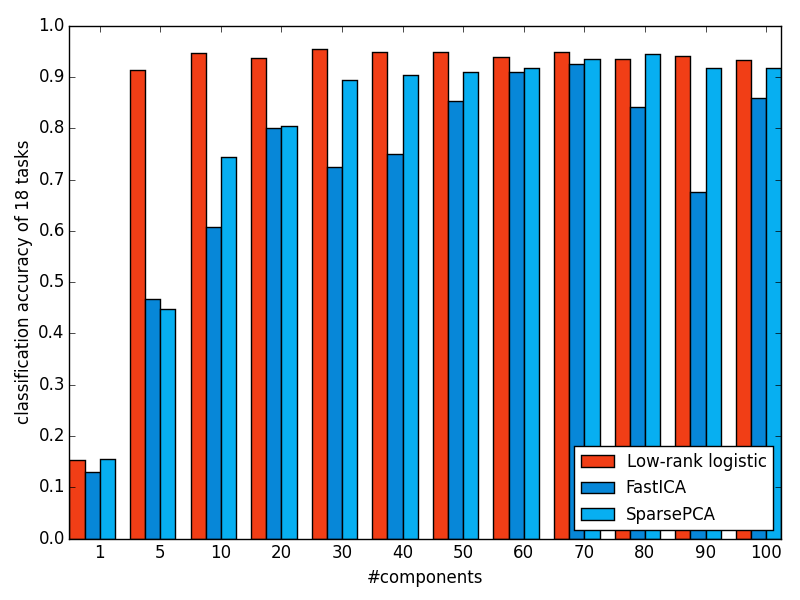
\includegraphics[width=0.48\textwidth]{fig001}
  \caption {\textbf{Integrated versus serial decomposition and classification}\\
  Depicts the out-of-sample performance of 18-task classification based on
	HCP task activity maps. Data reduction and classification
	was performed simultaneously (Low-rank logistic regression, red) or serially
	(ICA and SparsePCA, blue)}
\end{wrapfigure}


%
\section{Methods}
%

Data was drawn from 498 unrelated, healthy HCP participants.
All provided informed consent to the Washington
University in St. Louis institutional review board. HCP tasks 
were selected that feature known suitability as localizers
and reliability
across participants \citep{barch2013}.
Mostly block-design, but also event-related, paradigms were
administered on 1) working memory/cognitive control processing, 2)
incentive processing, 3) visual and somatosensory-motor processing,
4) language processing (semantic and phonological processing),
5) social cognition, 6) relational processing, and 7) emotional
processing. All data were acquired on the same Siemens Skyra 3T scanner.
Whole-brain EPI acquisitions were acquired with a
32 channel head coil (TR=720ms, TE=33.1ms, flip angle=52°, BW=2290Hz/Px,
in-plane FOV=$280\times180$mm, 72 slices, 2.0mm isotropic voxels).
The “minimally preprocessed” pipeline \citep{glass13} includes
gradient unwarping, motion correction, fieldmap-based EPI distortion
correction, brain-boundary-based registration of EPI to structural
T1-weighted scan, non-linear (FNIRT) registration into MNI space,
and grand-mean intensity normalization. Activation maps were spatially
smoothed by a Gaussian kernel of 4mm (FWHM). A general linear model (GLM) was
implemented by FILM from the FSL suite with model regressors from convolution
with a “canonical” hemodynamic response function and from temporal derivatives.
HCP tasks were conceived to modulate activation
in a maximum of different brain regions and neural systems. Indeed, at
least 70\% of the participants showed consistent brain activity in
contrasts from the task battery, which certifies excellent
coverage \citep{barch2013}.
In sum, the HCP task dataset incorporated 8650 first-level activity maps
from 18 diverse paradigms administered to 498 participants.
All maps were downsampled to a common 36x43x36 space of
5mm isotropic voxels and gray-matter masked (at least 10\%).
All analyses were based on task maps of
13,657 voxels representing Z values in gray matter.
\linebreak

Unsupervised and supervised learning were combined into a low-rank logistic
regression problem. The 13,657 z values from each activity map were
subject to a first linear
projection into Z latent components (i.e., 1, 5, 10, .., 100).
These hidden brain networks
loadings were subsequently projected into the 18 class space for multinomial
logistic regression. The goal was to find the two weight matrices
(input-to-hidden: 13,657 x Z and hidden-to-output: Z x 18) and their
corresponding bias vectors. Non-linearities were not applied on the
transformation results. Weights and biases were initialized by Gaussian
random noise. Gradient descent updated these matrices and vectors in each
iteration (100 samples per batch, 250 epochs). Using the chain rule, the
partial
derivates for the update were computed for the transformation into the
latent space and the subsequent transformation into the class space. We choose
the RMSprop algorithm \citep{dauphin15} with an initial learning rate of
0.01. Early stopping ensured that the best weight matrices/vectors were
retained in each epoch cycle. This was evaluated by the prediction
accuracy on a validation set (10\% of the training data) at each iteration.
\linebreak

This approach was benchmarked against independent dimensionality reduction and
learning of a classification function. Data reduction was performed on one
half of the data by ICA and SPCA.
ICA unmixed the
BOLD signals into separate spatial components
by minimizing their mutual information \citep{hyvarinen2000}.
This iterative blind source separation was
realized by a parallel FASTICA implementation (200 maximum iterations,
per-iteration tolerance of 0.0001,
initialized by a random mixing matrix, preliminary whitening).
SPCA separated the BOLD signals into
network components with few regions, which scales well to 
large datasets \citep{varoqu2011}.
This regression-type optimization problem constrained by
$\ell_1$-penalty in an implementation
without orthogonality assumptions
(1000 maximum iterations, per-iteration tolerance of 1 * 10\textsuperscript{-8}, sparsity
alpha=1, ridge-shrinkage at 0.01, Lasso path computed with coordinate
descent). Each linear decomposition revealed the specified number of
latent network components in one half the HCP data.
\linebreak
The extracted hidden network components were subsequently used
to reduce the remain half of task maps to a considerably smaller number of component
loadings. 13,657 voxels were thus condensed into 1, 5, 10, .., 100
measures of network involvement using ridge regression
(regularization alpha parameter=0.001, using
Cholesky solver). Multinomial logistic regression was finally performed on the
brain network loadings to learn classifying the 18 cognitive tasks.
Importantly, in all approaches, the final classification models were tested
on an unseen test set (10\% of data).
\linebreak

All analysis scripts that produced the results are accessible online
(\url{http://github.com/banilo/prni2015}).


\begin{figure*}
  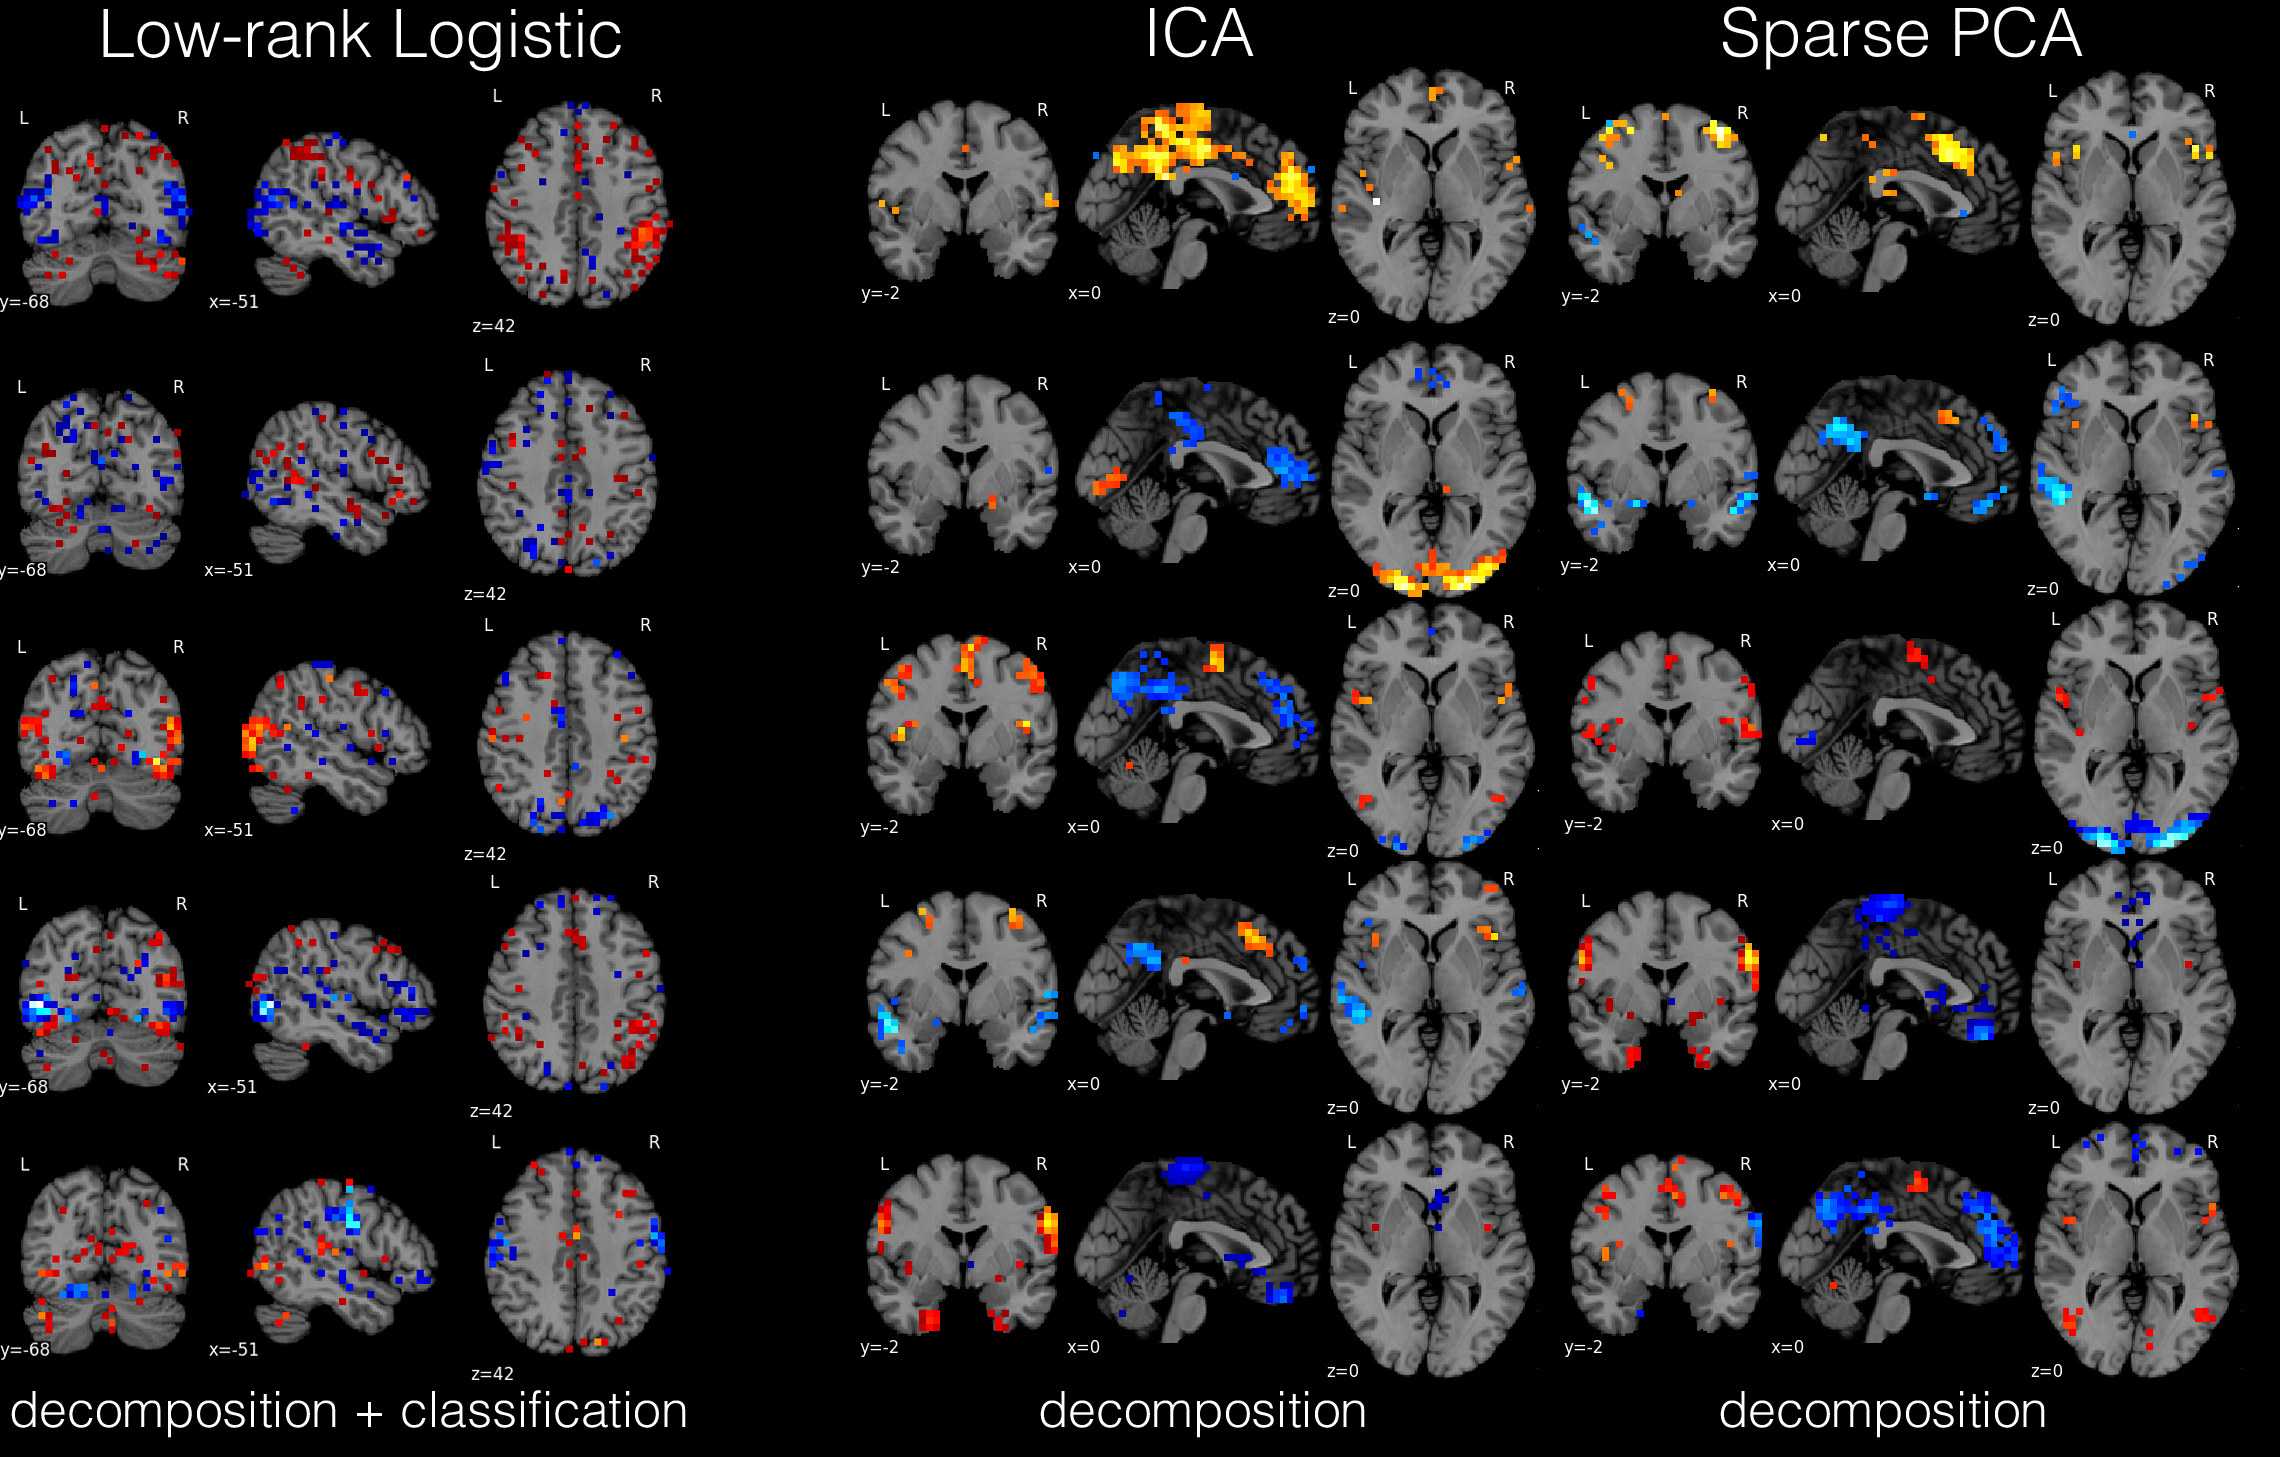
\includegraphics[width=0.98\textwidth]{fig002}
  \caption {\textbf{Decomposition into 5 networks}}
\end{figure*}

\section{Results}
Low-rank regression outperformed serial ICA/SparsePCA and logistic regression.



\section{Discussion}
%

-hypothesis space includes sparse PCA and PCA but not ICA since no
linearity


- if linearity, then would be closer to the notion of 1-hidden layer neural
network rather than low-rank logistic regression



%
\paragraph{Acknowledgment}
{\small
Data were provided the Human Connectome Project.
}

%
% ---- Bibliography ----
%
\bibliographystyle{IEEEtran}
\bibliography{prni_refs}
%
\end{document}
